\documentclass[class=article, crop=false]{standalone}
\usepackage{standalone}
\usepackage{labor}
\usepackage{pageslts}
\usepackage{hyperref}
\usepackage{booktabs}
\usepackage{listings}
\usepackage[latin1]{inputenc}
\usepackage{tikz}
\usetikzlibrary{shapes,arrows}

% Verwendung von Umlauten
\usepackage[ngerman]{babel}
% Auf Windows folgendes Paket verwenden
%\usepackage[ansinew]{inputenc}
% Auf Mac folgendes Paket verwenden
%\usepackage[applemac]{inputenc}

\lstset{ 
	language=python,
	basicstyle=\footnotesize\ttfamily,
	%basicstyle=\ttfamily
	numbers=left,
	stepnumber=1,
	tabsize=4,
	frame=lines,
}

\renewcommand{\lstlistingname}{Code}% Listing -> Algorithm

\begin{document}

	\pagenumbering{arabic}
	\newpage
	\thispagestyle{empty}
	
	\begin{center}
		\normalfont \sffamily 
		\begin{tabular*}{\textwidth}{@{\extracolsep{\fill}}lr@{}}
			{INSTITUT F\"{U}R } & {\small Appelstra\ss e 9A} \\
			{INFORMATIONSVERARBEITUNG} & {\small 30167 Hannover} \\
			{\small LEIBNIZ UNIVERSIT\"{A}T HANNOVER} & 
		\end{tabular*}
	\end{center}
	
	\vspace{1.5cm}
	\begin{center}
	{\Large Labor zur Vorlesung\\[.2cm] {\normalfont\bfseries Digitale Bildverarbeitung}}
	\end{center}

	
	%\addcontentsline{toc}{}{Titelblatt}
	
	\vspace{2cm}
	
	\begin{tabular}{@{}p{4cm}l}
		Datum:                  & XX.XX.XXXX \\
		Uhrzeit:                & XX:XX \\
		Anzahl der Bl\"{a}tter: & \lastpageref*{LastPages} (einschlie\ss{}lich Deckblatt)
		
	\end{tabular}
	
	\vspace{3cm}
	
	\begin{tabular}{@{}p{4cm} l }
	{\normalfont\bfseries Name:} & 	{\normalfont\bfseries Matrikelnummer:}\\ 
	$\underline{\hspace{5cm}}$  \hspace{0.5cm}& $\underline{\hspace{5cm}}$ \\
	$\underline{\hspace{5cm}}$ \hspace{0.5cm}& $\underline{\hspace{5cm}}$\\
	$\underline{\hspace{5cm}}$ \hspace{0.5cm}& $\underline{\hspace{5cm}}$\\
	\end{tabular}
		
	\vspace{2.0cm}
	
	Die Bearbeitung der Aufgaben erfolgt selbstst�ndig in Kleingruppen. Alle Gruppenmitglieder sollen Arbeitsaufwand in gleicher Gr��enordnung einbringen. Betrugsversuche werden geahndet. 


\tableofcontents

\newpage
\section{Einleitung}
Digitale Bildverarbeitung wird unter anderem in industriellen Prozessen, medizinischen Verfahren oder in Multimedia-Produkten angewandt. In diesem Labor soll eine beispielhafte Multimedia-Anwendung entwickelt werden, die �ber das Labor hinaus als erheiterndes Demonstrationsobjekt f�r Bildverarbeitung in Videokonferenzen genutzt werden kann. Als Inspiration dient ein Effekt aus der Filmreihe \glqq Harry Potter\grqq .

\begin{figure}
	\centering
	\begin{minipage}{.45\textwidth}
		\centering
		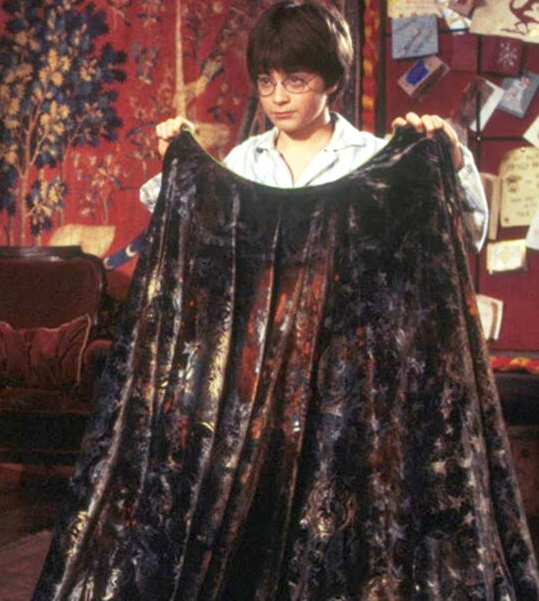
\includegraphics[width=.6\linewidth]{fig/harry1.jpg}
		\caption{Harry Potter ohne magischen Tarnumhang}
		\label{fig:harry1}
	\end{minipage}%
	\hspace{0.5cm}
	\begin{minipage}{.45\textwidth}
		\centering
		
\includegraphics[width=.6\linewidth]{fig/harry2.jpg}
		\caption{Harry Potter mit magischem Tarnumhang}
		\label{fig:harry2}
	\end{minipage}
\end{figure}

Die Abbildungen \ref{fig:harry1} und \ref{fig:harry2} zeigen Harry Potter ohne
\footnote{\url{https://assets.cdn.moviepilot.de/files/8a2cc0d2eb31c41136fb2be242540606dcd50821980e830481404b276065/fill/1280/614/Harry\%20Potter\%20Tarnumhang.jpg}} 
und mit\footnote{\url{https://www.tres-click.com/wp-content/uploads/2019/06/harry-potter-tarnumhang.gif}}
verzauberten Tarnumhang, welchen den Tr�ger des Umhangs verschwinden lassen kann. In diesem Labor entwickeln Sie eine Bildverarbeitungs-Pipeline, mit welcher dieser Effekt mit einer einfachen Webcam simuliert werden kann. Sie festigen den Umgang mit

\begin{itemize}
	\item Rauschunterdr�ckung
	\item Histogrammen 
	\item verschiedenen Farbr�umen
	\item Erosion und Dilatation
	\item Schwellwertverfahren 
\end{itemize}

und �ben gleichzeitig den Umgang mit der Programmiersprache Python.

\newpage
\subsection{Vorbereitung}
F�r das Labor wird ein Rechner mit Betriebssystem Windows, Linux-Ubuntu oder Mac ben�tigt. Zus�tzlich muss eine Webcam vorhanden sein (im Laptop integriert oder extern).
Melden Sie sich \textbf{vorab} bei dem Betreuer des Labors, sollte Ihnen eines der ben�tigten Mittel nicht zur  Verf�gung stehen.


Um an dem Labor erfolgreich teilnehmen zu k�nnen, muss die zu nutzende Programmierumgebung vorbereitet werden. Sollten Sie an der praktischen �bung zur Vorlesung \textit{Digitale Bildverarbeitung} teilgenommen haben, ist die erforderliche Programmierumgebung sowie der Programmcode wahrscheinlich bereits installiert und eingerichtet. Ansonsten befolgen Sie die Installationsanweisungen auf \url{https://github.com/TimoK93/Digitale-Bildverarbeitung} im Bereich \textit{0\_Einf�hrung}. Die Installation des Streaming Programms zur Erstellung einer virtuellen Kamera ist dabei optional und nicht verpflichtend.

Nachdem Sie die Installation vollendet haben, �ffnen Sie die Programmierumgebung, sodass Ihr Bildschirm �hnliches zu Abbildung \ref{fig:pycharm} anzeigt.

\begin{figure}
	\centering
	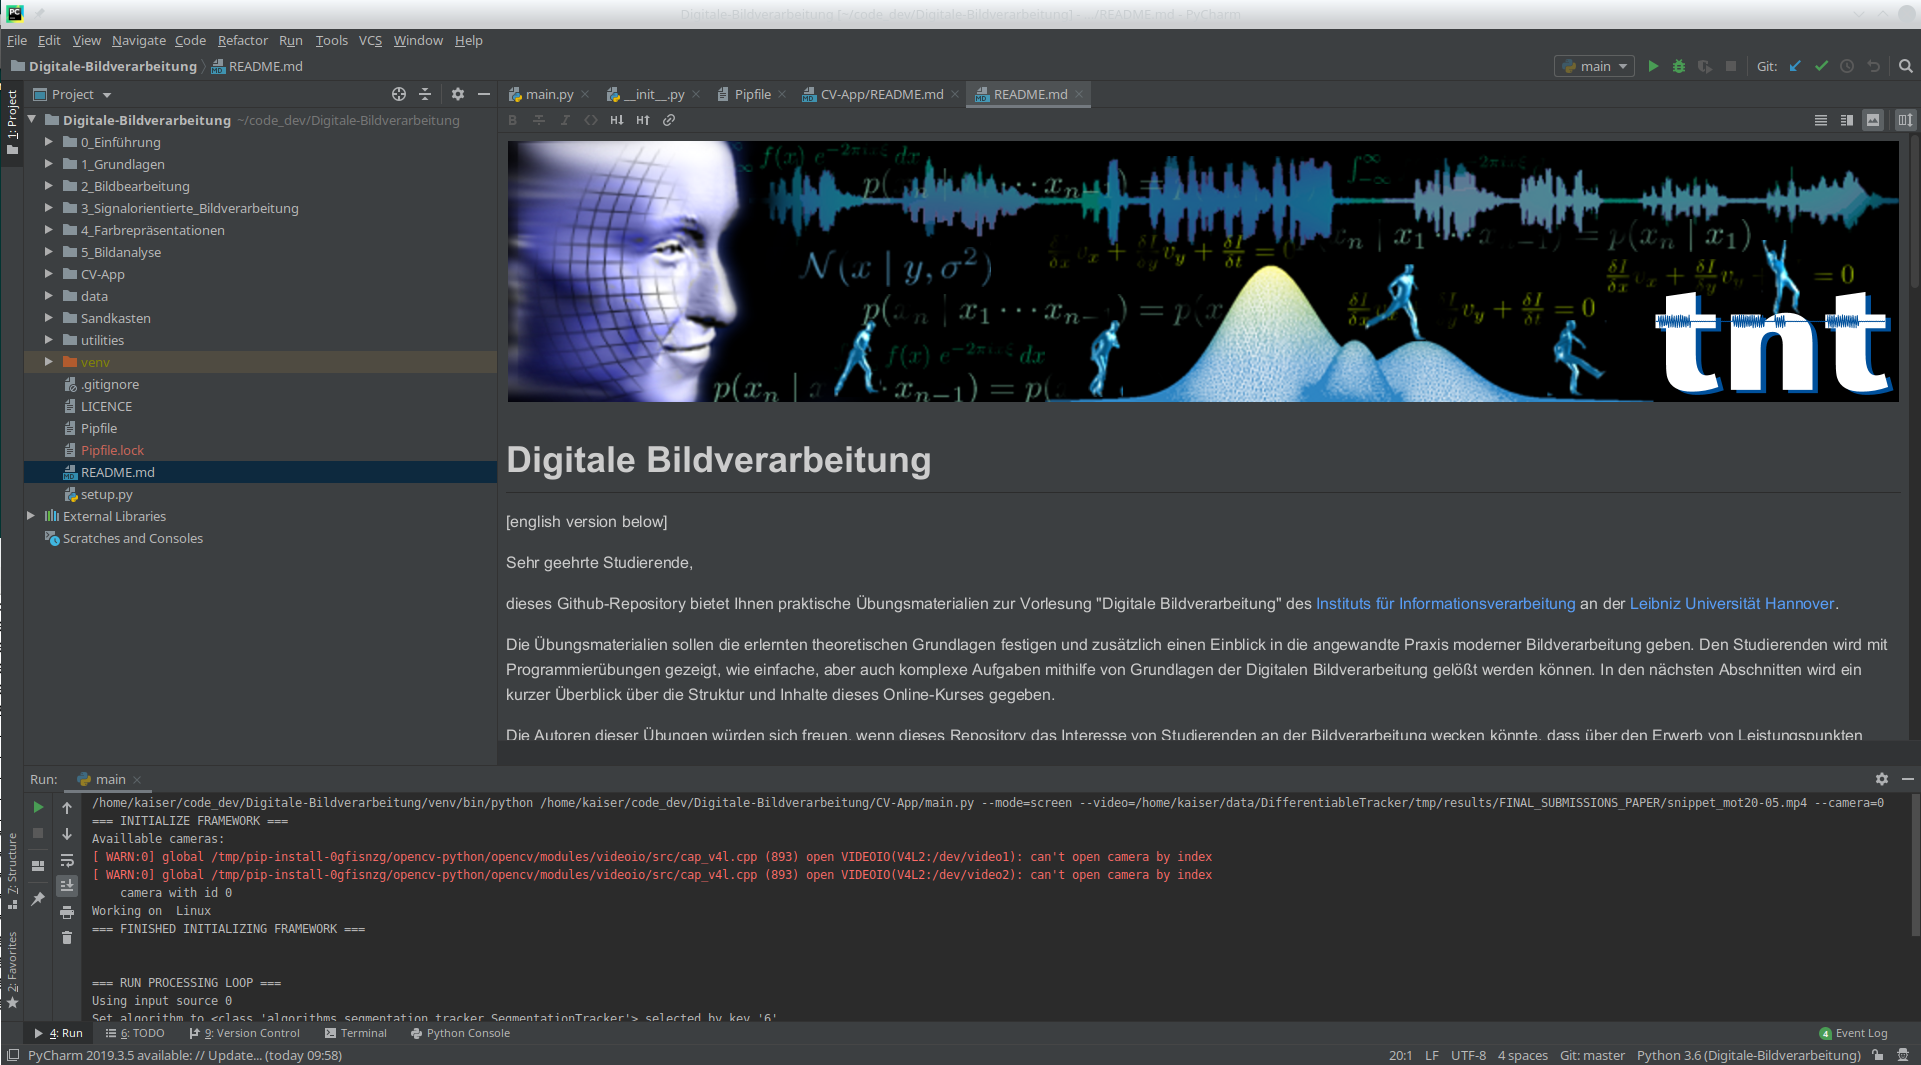
\includegraphics[width=\linewidth]{fig/pycharm.png}
	\caption{Programmierumgebung in PyCharm}
	\label{fig:pycharm}
\end{figure}

Machen Sie sich als n�chstes mithilfe der Beschreibung in Kapitel \ref{sec:Programmierumgebung} mit der Programmierumgebung vertraut. 



\newpage
\subsection{Programmierumgebung}  
\label{sec:Programmierumgebung}
In der Programmierumgebung ist das Hauptprogramm bereits soweit vorbereitet, sodass Sie einen Videostream aus Ihrer Kamera auslesen, darauf einen vorbereiteten Beispielalgorithmus anwenden und diesen anzeigen k�nnen. In diesem Kapitel wird kurz erl�utert, wie Sie diese Bildverarbeitungs-Pipeline starten und eigene Algorithmen integrieren k�nnen.

\paragraph*{Starten der Bildverarbeitungs-Pipeline.} �ffnen Sie die Datei \mbox{\textit{./CV-App/main.py}} in PyCharm und klicken Sie mit der rechten Maustaste in den Programmcode. �ffnen Sie dann das Fenster \textit{Modify Run Configuration...} wie in Abbildung \ref{fig:run_config} dargestellt. In dem Feld \textit{Parameter} k�nnen Sie zus�tzliche Argumente in die Umgebung eingeben. Argumente werden dabei im Schema \textit{--Argument1 Value1 --Argument2 Value2} eingegeben. Die einzustellenden Parameter k�nnen Sie aus der Tabelle \ref{tab:parameter} entnehmen. Wenn Sie keine Argumente w�hlen, werden die Standard Einstellungen gew�hlt.

\begin{table}
	\centering
	\caption{Argumente f�r die Programmausf�hrung}
	\begin{tabular}[h]{c | l| c}
		Argument & Werte & Default-Wert \\ \toprule
		 \textit{camera}	 & -1, 0, 1, \ldots (-1 �ffnet ein Video) & 0 \\
		 \textit{mode}	 & \textit{virtual\_cam} (virtuelle Kamera), \textit{screen} (nur Fenster)&  \textit{virtual\_cam} \\
		 \textit{video}	 & Pfad zu Video, wenn \textit{camera} den Wert $-1$ hat. & - \\
	\end{tabular}
		\label{tab:parameter}
\end{table}

\begin{figure}
	\centering
	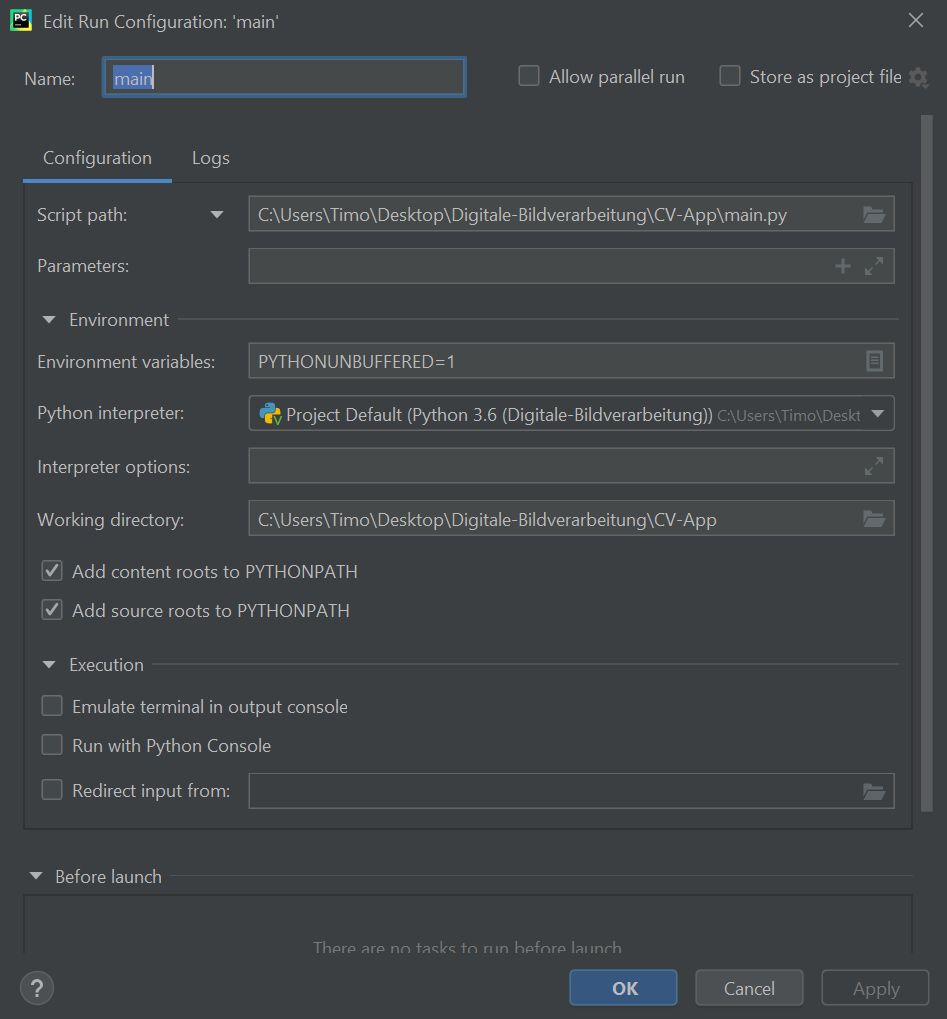
\includegraphics[width=0.65\linewidth]{fig/Run-Configs.png}
	\caption{Run Configuration in PyCharm}
	\label{fig:run_config}
\end{figure}

 Sie k�nnen das Programm nun mit \textit{Run} starten. Kurz nach dem Start sollten Sie ein Fenster mit dem Videostream aus Ihrer Kamera sehen. Durch das Bet�tigen verschiedener Tasten auf der Tastatur (z.B.\ Taste 1 oder 2) k�nnen Sie verschiedene Algorithmen aktivieren. Sie sehen das Ergebnis direkt in dem ausgegebenem Videostream. Wichtig: Das Programm reagiert nur auf Tastendr�cke, wenn das Videostream-Fenster im Vordergrund ihres Bildschirms ist.
 
 
 \paragraph*{Eigene Algorithmen einbinden.} F�r Sie sind nur die Dateien im Dateipfad \mbox{ \textit{./CV-App/algorithms}} relevant. Beispielhaft erstellen Sie im Folgenden den Algorithmus \textit{YourAlgorithm}.
 
 Erstellen Sie eine Datei \textit{your\_algorithm.py} und kopieren Sie den Inhalt aus dem Code \ref{lst:code2}. In der Funktion \textit{\_\_init\_\_(self)} k�nnen Sie dauerhafte Variablen definieren. Die Funktion \textit{process(self, img)} verarbeitet das Eingangsbild \textit{img} und gibt es am Ende modifiziert wieder aus (Hinweis: Ein und Ausgangsbild m�ssen gleich gro� sein!). Die Funktion \textit{mouse\_callback(self, ...)} reagiert auf Aktionen der Maus, wie zum Beispiel einem Mausklick an der Position x und y. So k�nnen Sie mit ihrem Algorithmus interagieren. Sie k�nnen sich einige Beispielalgorithmen in dem Ordner \textit{./CV-App/algorithms} zur Veranschaulichung ansehen. Der Algorithmus in \textit{white\_balancing.py} veranschaulicht alle Funktionen mit Algorithmen der Klasse \textit{Algorithm}.
 
  % Settings for listings
 \lstset{caption={Eigener Algorithmus in \textit{your\_algorithm.py}}}
 \lstset{label={lst:code2}}
 \begin{lstlisting}
import cv2
import numpy as np
from . import Algorithm

class YourAlgorithm(Algorithm):
    def __init__(self):
      self.some_persistent_value = "i_am_alwys_existing"
 
    def process(self, img):
        print(self.some_persistent_value)
        return img
 
    def mouse_callback(self, event, x, y, flags, param):
        if event == cv2.EVENT_LBUTTONUP:
            print("A Mouse click happend! at position", x, y)	 
 \end{lstlisting} 
 
 \newpage
 Um Ihren Algorithmus nun mit einer Aktivierungstaste-Taste zu verlinken, �ffnen Sie die Datei \textit{\_\_init\_\_.py}. Am Ende der Datei ist eine Verlinkung der Algorithmen zu bestimmten Tasten zu sehen (siehe Code \ref{lst:code1}).. In dem Beispiel in Code \ref{lst:code1} ist Ihr neuer Algorithmus \textit{YourAlgorithm} importiert und an die Taste 3 verlinkt. 
 
 % Settings for listings
 \lstset{caption={Verlinkung der Algorithmen in \textit{\_\_init\_\_.py}}}
 \lstset{label={lst:code1}}
 \begin{lstlisting}
from .image_to_gray import ImageToGray
from .image_to_hue import ImageToHue
from .your_algorithm import YourAlgorithm

algorithms = dict()
algorithms["0"] = Algorithm
algorithms["1"] = ImageToGray
algorithms["2"] = ImageToHue
algorithms["3"] = YourAlgorithm
 \end{lstlisting} 
 
 Nach Neustart des Programms durch erneute Bet�tigung der \textit{Run} Funktion, ist Ihr Algorithmus durch bet�tigen der Taste 3 zug�nglich.
\newpage
\section{Aufgabe}
Das Ziel ist die Detektion des \glqq magischen Umhangs\grqq\ sowie das k\"unstliche Entfernen eines Objektes im Vordergrund. Daf\"ur werden in diesem Labor drei Arbeitspakete bearbeitet: Die Vorverarbeitung, die Farbanalyse der Szene und die Segmentierung des Umhangs. Eine Skizze der Bildverarbeitungs-Pipeline ist in Abbildung \ref{fig:skizzepipeline} dargestellt.

\begin{figure}
\centering

\tikzstyle{decision} = [diamond, draw, fill=blue!20, text width=4.5em, text badly centered, node distance=3cm, inner sep=0pt]
\tikzstyle{block} = [rectangle, draw, fill=blue!20, text width=8em, text centered, rounded corners, minimum height=4em]
\tikzstyle{line} = [draw, -latex']
\tikzstyle{cloud} = [draw, ellipse,fill=red!20, node distance=4cm, minimum height=2em]
\begin{tikzpicture}[node distance = 2cm, auto]
   % Place nodes


\node [block, fill=green!20] (Rauschreduktion) {Rauschreduktion};
\node [block, fill=green!20, below of=Rauschreduktion] (Histogramm) {Histogramm Spreizung};
\node [block, fill=yellow!20, below of=Histogramm] (Farbanalyse) {Farbanalyse};
\node [block, fill=blue!20, below of=Farbanalyse] (Schwellwertverfahren) {Schwellwert-verfahren};
\node [block, fill=blue!20, below of=Schwellwertverfahren] (Maske) {Bin\"armasken-Optimierung};
\node [block, fill=blue!20, below of=Maske] (Bildmodifizierung) {Bildmodifizierung};
\node [cloud, left of=Rauschreduktion] (Webcam) {Webcam};
\node [cloud,right of=Bildmodifizierung] (Output1) {Screen};
\node [cloud,below of=Output1, node distance=1.5cm] (Output2) {Virtuelle Kamera};
\node [cloud,left of=Bildmodifizierung] (Input2) {Maus-Events};
%\node [cloud, left of=init] (expert) {expert};
%\node [cloud, right of=init] (system) {system};
%\node [block, below of=init] (identify) {identify candidate models};
%\node [block, below of=identify] (evaluate) {evaluate candidate models};
%\node [block, left of=evaluate, node distance=3cm] (update) {update model};
%\node [decision, below of=evaluate] (decide) {is best candidate better?};
%\node [block, below of=decide, node distance=3cm] (stop) {stop};


% Draw edges
\path [line] (Webcam) -- (Rauschreduktion);
\path [line] (Rauschreduktion) -- (Histogramm);
\path [line] (Histogramm) -- (Farbanalyse);
\path [line] (Farbanalyse) -- (Schwellwertverfahren);
\path [line] (Schwellwertverfahren) -- (Maske);
\path [line] (Maske) -- (Bildmodifizierung);
\path [line] (Bildmodifizierung) -- (Output1);
\path [line,dashed] (Bildmodifizierung) -- (Output2);
\path [line] (Input2) -- (Bildmodifizierung);
%\path [line] (identify) -- (evaluate);
%\path [line] (evaluate) -- (decide);
%\path [line] (decide) -| node [near start] {yes} (update);
%\path [line] (update) |- (identify);
%\path [line] (decide) -- node {no}(stop);
%\path [line,dashed] (expert) -- (init);
%path [line,dashed] (system) -- (init);
%\path [line,dashed] (system) |- (evaluate);

\end{tikzpicture}
\caption{Bildverarbeitungs-Pipeline}
\label{fig:skizzepipeline}
\end{figure}

Die Szene f\"ur diesen Versuch wird durch Sie definiert: W"ahlen Sie sich eine eint"onige, m"oglichst monotone  Umgebung als Szene f\"ur diesen Versuch. Der \glqq magische Umhang\grqq\ wird dann durch einen einfarbigen Gegenstand (es muss kein Umhang sein!) realisiert. Achten Sie darauf, dass sich der Umhang farblich von der Szene unterscheidet. Je st"arker der Kontrast zwischen \glqq Umhang\grqq\ und Szene ist, desto besser l"asst sich dieser Versuch durchf"uhren.  


Im folgenden finden Sie detaillierte Beschreibungen der Arbeitspakete. Bitte beantworten Sie die vorhandenen Fragen und erstellen Sie ggf.\ geforderten Code oder Abbildungen. Die Bearbeitung der Fragen kann entweder innerhalb dieses Latex Dokuments, oder in einem separatem PDF geschehen. 




\newpage
\subsection{Vorverarbeitung}
Um die folgende Verarbeitung der Bilder zu vereinfachen und robuster zu gestalten, sollen Sie den Videostream mit einem Preprocessing vorverarbeiten. 
Binden Sie daf�r die Datei \textit{./CV-App/algorithms/invis\_cloak.py} in den Algorithmus ein, wie in der Einleitung beschrieben.
Die folgenden Aufgabenstellungen sind in den daf�r vorgesehenen Funktionen zu bearbeiten.
%Erstellen Sie daf�r einen neuen Algorithmus, wie in der Einleitung beschrieben. 

\subsubsection{Rauschreduktion}
Jeder Farbwert eines Pixels $I_k(x, y) \in \{0, \ldots, 255 \}$ mit $k\in \{R, G, B\}$ wird auf dem Kamerasensor durch einen elektrischen Halbleiter physikalisch gemessen. Je nach Sensorqualit�t und Lichtbedingungen wirkt dabei ein unterschiedlich ausgepr�gtes Rauschen auf die Farbwerte ein, sodass der zur Verf�gung stehende Farbwert als Summe

\begin{equation}
I_k(x, y) = I^*_k(x, y) + r(x, y)   
\end{equation}

aus realem Farbwert $I^*_k(x, y) $ und statistischem Rauschen $r(x,y)$ modelliert werden kann. Das Rauschen $r$ kann als normalverteilt um den Mittelwert $0$ angenommen werden. Unter den Annahmen, dass die Kamera statisch montiert ist und in der aufgenommenen Szene keine Ver�nderung passiert,  kann der Zusammenhang

\begin{equation}
	\overline{I}_{k,t}(x, y) =   \lim_{N\rightarrow \infty} \frac{1}{N + 1} \sum_{n=0}^N I^*_{k,t-n}(x, y) + r_{t-n}(x, y)  \stackrel{!}{=} I^*_{k,t}  
\end{equation}

f�r die Mittelwertbildung �ber lange Zeitr�ume formuliert werden. Dabei beschreibt $t$ den Zeitpunkt, zu dem der entsprechende Wert gemessen wurde.

Um die Bildqualit�t zu erh�hen, soll der Einfluss von $r$ reduziert werden. Es soll daf�r angenommen werden, dass die Kamera statisch ist und kaum Bewegung in zwei aufeinander folgenden Bildern vorhanden ist. 
Implementieren Sie die Mittelwertbildung mit einer variablem Bildreihe $N$ (default: $N=1$) und geben Sie das Bild aus. \\
Um zu pr�fen wie das Bild auf Pixelebene arbeitet, kann die Variable \textit{plotNoise} in der Funktion \textit{process()} auf \textit{True} gesetzt werden.
Es werden zwei zus�tzliche Plots ausgegeben, in der ein Bildausschnitt des Zentrums vor- und nach der Rauschunterdr�ckung vergr��ert dargestellt werden.


\paragraph*{Aufgabe 1}
Geben Sie Ihren Code an und beschreiben Sie ihn. Geben Sie nur relevante Code Bereiche an!
 \lstset{caption={Vorverarbeitung, Aufgabe 1}}
\begin{lstlisting}
# Your code!
\end{lstlisting} 

\paragraph*{Aufgabe 2}
Nennen Sie Vor und Nachteile, wenn $N$ vergr��ert werden w�rde. Sollte $N$ in dieser Anwendung vergr��ert werden?

\paragraph*{Aufgabe 3}
Beschreiben Sie eine weitere Methode zur Rauschreduktion. Diskutieren Sie dabei Vor- oder Nachteile!

\subsubsection{Histogramm Spreizung}
Pixel k�nnen in unserer Anwendung Werte von $I_k(x,y) \in \{ 0, \ldots , 255 \}$ annehmen. Dieser Wertebereich wird nicht zwangsl�ufig ausgenutzt. Um das zu �ndern, soll eine Histogramm Spreizung auf den Helligkeitsinformationen der Pixel durchgef�hrt werden.

Implementieren Sie zus�tzlich zur Rauschreduktion eine Histogramm Spreizung, indem sie (1) das Rausch-reduzierte Eingangsbild in den HSV-Farbbereich transformieren und (2) die Rechenvorschrift~\ref{equ:histogramm-equalization} auf den V-Kanal anwenden. Transformieren Sie das Bild dann (3) wieder in den RGB Farbraum.

\begin{equation}
\label{equ:histogramm-equalization}
I_V^{\textnormal{new}}(x,y) = \frac{I_{V}(x,y) - \min I_{V}}{\max I_{V} - \min I_{V}} \cdot 255
\end{equation}

\textbf{Hinweis:} Nutzen Sie die Befehle \textit{cv2.cvtColor(img, cv2.COLOR\_BGR2HSV)} beziehungsweise \textit{cv2.cvtColor(img, cv2.COLOR\_HSV2BGR)}.


\paragraph*{Aufgabe 4}
Geben Sie Ihren Code an und beschreiben Sie ihn. Geben Sie nur relevante Code Bereiche an!
\lstset{caption={Vorverarbeitung, Aufgabe 4}}
\begin{lstlisting}
# Your code!
\end{lstlisting} 

\paragraph*{Aufgabe 5}
Warum ist es sinnvoll, den gesamten Wertebereich f�r die Darstellung von Videos in Multimedia-Anwendungen auszunutzen?
\newpage
\subsection{Farbanalyse}
Die Zugrundeliegende Aufgabe ist die Detektion des \glqq magischen Umhangs\grqq , der Objekte verschwinden lassen kann. Der Umhang kann durch eine einfarbige Decke modelliert werden. Sollte keine einfarbige Decke vorhanden sein, kann ebenfalls ein einfarbiges Blatt Papier zur Hilfe genommen werden.

Das Ziel des Arbeitspakets \glqq Farbanalyse\grqq\ ist es, die farblichen Eigenschaften der Szene, sowie des \glqq magischen Umhangs\grqq\ zu untersuchen. Daf�r sollen die Histogramme einzelner Farbkan�le mit und ohne Umhang erstellt und analysiert werden.

\textbf{Hinweis:} Versuchen Sie von nun an die Position der Kamera nicht mehr zu ver�ndern!

\subsubsection{RGB}
Einzelne Pixel werden durch drei Werte repr�sentiert. Jeweils ein Wert $I_k(x, y) \in \{0, \ldots, 255 \}$ mit $k\in \{R, G, B\}$  beschreibt die einfallende Lichtmenge f�r die Farben Rot, Gr�n und Blau. In OpenCV werden Bilder im BGR Format repr�sentiert. Die Verteilung der Farbwerte kann durch ein Histogramm dargestellt werden. Ein Histogramm 
\begin{equation}
h(v) = |I_v| 
\end{equation}
beschreibt die Anzahl der Menge Pixel $I_v$ im Bild, welche den Wert $v$ haben. In OpenCV kann das Histogramm mit der Funktion \textit{cv2.calcHist(image, [Kanal], None, [histSize], histRange, False)} berechnet werden. Dabei gibt \textit{histSize} die Anzahl der Intervalle und $\textit{histRange} = (0, 256)$ die obere und untere Schrank f�r den zu betrachtenden Wertebereich an.

Implementieren Sie in Ihren Algorithmus eine Funktion, mit dem Sie per Mausklick das aktuelle Bild speichern k�nnen. Des Weiteren soll bei Bet�tigung des Mausklicks ein Histogramm f�r jeden Farbkanal des RGB-Bilder erstellt und abgespeichert werden. Mit Hilfe des Code-Schnipsel in Code \ref{lst:Histogramm} kann ein Histogramm angezeigt oder gespeichert werden!

\begin{lstlisting}[caption={Histogrammberechnung mit \textit{matplotlib}},label={lst:Histogramm}]
import cv2 
from matplotlib import pyplot as plt

channel = 0 #[0:B, 1:G, 2:R]
hist_size = 256
hist_range = [0,256]
histr = cv2.calcHist([img], [channel], None, [hist_size], hist_range)
plt.plot(histr, color = "b")
plt.xlim([0,256])
plt.savefig('the_path_to_store.png')
plt.show()
\end{lstlisting} 

Nehmen Sie mit dem fertig implementierten Code ein Bild und die Histogramme in der von Ihnen pr�ferierten Szene auf. Nehmen Sie sich darauf den \glqq magischen Umhang\grqq zur Seite und halten ihn sehr gut sichtbar vor die Kamera. Nehmen Sie auch jetzt ein Bild mit den Histogrammen auf. Die Kamera sollte sich zwischen den beiden Bildern nicht bewegen.


\paragraph*{Aufgabe 1}
Geben Sie Ihren Code an und beschreiben Sie ihn. Geben Sie nur relevante Code Bereiche an! Geben sie zus�tzlich die aufgenommenen Bilder und die erstellten Histogramme an.
  
\lstset{caption={Farbanalyse, Aufgabe 1}}
\begin{lstlisting}
# Your code!
\end{lstlisting} 

\paragraph*{Aufgabe 2}
Interpretieren Sie die Ver�nderungen zwischen den  Histogrammen mit und ohne \glqq magischen Umhang\grqq . Verhalten sich die einzelnen Kan�le gleich? Lassen sich Bereiche in den Histogrammen herausstellen, die dem Umhang zuzuordnen sind? Diskutieren Sie Ihre Beobachtungen.

\subsubsection{HSV}
Erweitern Sie ihren vorherigen Code um eine Farbkonvertierung in den HSV-Farbraum. F�hren Sie die Konvertierung vor Erstellung der Histogramme durch und wiederholen Sie die Schritte aus dem vorherigen Aufgabenteil. 

\paragraph*{Aufgabe 3}
Geben sie die aufgenommenen Bilder und die erstellten Histogramme an.

\paragraph*{Aufgabe 4}
Interpretieren Sie die Ver�nderungen zwischen den  Histogrammen mit und ohne \glqq magischen Umhang\grqq . Verhalten sich die einzelnen Kan�le gleich? Lassen sich Bereiche in den Histogrammen herausstellen, die dem Umhang zuzuordnen sind? Diskutieren Sie Ihre Beobachtungen.

\paragraph*{Aufgabe 5}
Versuchen Sie mit den gegebenen Histogrammen Wertebereiche zu finden, mit denen Sie den \glqq magischen Umhang\grqq\ segmentieren k�nnten. Formulieren Sie eine Regel in dem Format
\begin{equation}
\label{equ:segrule}
	S_\textnormal{Umhang} = \{ I(x, y)\ |\  \\  R_\textnormal{min} < I_R(x, y) <  R_\textnormal{max} \ \ \textnormal{und} \ \ \ldots \}  \quad ,
\end{equation}
wobei $S_\textnormal{Umhang}$ die Bin�rmaske beschreibt und $R_\textnormal{min}$ und $R_\textnormal{max}$ beispielhafte Schwellwerte f�r den Rot-Kanal sind.

\paragraph*{Aufgabe 6}
Worauf muss geachtet werden, wenn mit dem H-Kanal des HSV-Farbraums gearbeitet wird?
\newpage
\subsection{Segmentierung und Bildmodifizierung}
In diesem Arbeitspaket werden Sie auf Grundlage der vorherigen Analysen eine Segmentierung des magischen Umhangs realisieren. Anschlie�end werden Sie den segmentierten Bereich \glqq verschwinden\grqq\ lassen, indem sie ein statisches Bild des Hintergrunds auf diese Fl�chen einf�gen.


\subsubsection{Statisches Schwellwertverfahren}
Implementieren Sie die von Ihnen gefundene Regel nach Gleichung~\ref{equ:segrule}, um eine Bin�rmaske zu erhalten. Sie k�nnen die Randbedingungen wie im folgenden Code-Schnipsel \ref{lst:conditions} implementieren.

\begin{lstlisting}[caption={Benutzung von Randbedingungen mit \textit{numpy}}, label={lst:conditions}]
import cv2 
import numpy as np

channel1 = 0
lower_bound1, upper_bound1 = 15, 100
is_condition_1_true = (lower_bound1 < img[:, :, channel1]) * \
	(img[:, :, channel1] < upper_bound1)
channel2 = 1
lower_bound2, upper_bound2 = 65, 172
is_condition_2_true = (lower_bound2 < img[:, :, channel2]) * \
(img[:, :, channel2] < upper_bound2)

binary_mask = is_condition_1_true * is_condition_2_true
\end{lstlisting} 

Geben Sie die gefundene Bin�rmaske als Ausgangsbild auf dem Bildschirm aus. Sollten die gefundenen Wertebereich zu keinen sinnvollen Segmentierungen f�hren, d�rfen Sie Gleichung~\ref{equ:segrule} selbstverst�ndlich anpassen!

Implementieren Sie ebenfalls eine Mausklick-Funktion, mit der Sie das aktuelle Bild und die dazugeh�rige Bin�rmaske abspeichern k�nnen. F�r das Abspeichern von Bildern k�nnen Sie die Funktion \textit{cv2.imwrite(img, "path\_to\_store.png")} verwenden.

\paragraph*{Aufgabe 1}
Geben Sie Ihren Code an und beschreiben Sie ihn. Geben Sie nur relevante Code Bereiche an! Geben Sie ebenfalls das aufgenommene Bild sowie die dazugeh�rige Bin�rmaske an.

\lstset{caption={Segmentierung und Bildmodifizierung, Aufgabe 1}}
\begin{lstlisting}
# Your code!
\end{lstlisting} 

\subsubsection{Bin�rmaske}
Die in der vorherigen Aufgabe erhaltene Bin�rmaske ist ggf.\ ungeeignet f�r eine zufriedenstellende Segmentierung. Sie sollen die Maske nun optimieren. Wenden Sie daf�r das \textit{Opening} und \textit{Closing} auf die Bin�rmaske an.  Nutzen Sie die Funktionen \textit{cv2.erode(img, kernel)} und \textit{cv2.dilate(img, kernel)}. 

W�hlen Sie zum Schluss die gr��te zusammenh�nge Region segmentierter Pixel aus, und l�schen alle anderen Segmente. Folgender Code-Schnipsel~\ref{lst:contours} soll als Hilfestellung dienen. Recherchieren Sie ggf.\ im Internet.  

\lstset{caption={Konturfindung}}
\lstset{label={lst:contours}}
\begin{lstlisting}
(cnts, _) = cv2.findContours(
		binary_mask, cv2.RETR_LIST, cv2.CHAIN_APPROX_SIMPLE)
c = max(cnts, key = cv2.contourArea)
img = cv2.drawContours(img, [c], -1, color=255, -1)
\end{lstlisting} 

\paragraph*{Aufgabe 2}
Geben Sie Ihren Code an und beschreiben Sie ihn. Geben Sie nur relevante Code Bereiche an!
\lstset{caption={Segmentierung und Bildmodifizierung, Aufgabe 2}}
\begin{lstlisting}
# Your code!
\end{lstlisting} 

\paragraph*{Aufgabe 3}
Welche Probleme oder Fehler k�nnen in der Bin�rmaske vorkommen, die mit den Ma�nahmen beseitigt werden sollen?

\subsubsection{Bildmodifizierung}
Nach dem Fertigstellen der vorherigen Aufgabenstellungen sollten Sie nun eine Bin�rmaske erhalten, welche den \glqq magischen Umhang\grqq\ segmentiert. Die letzte Aufgabe befasst sich mit der Bildmodifizierung, welche den Eindruck verschwindender Objekte vermittelt.

Sie sollen nun folgende Funktionen implementieren: 

Erstellen Sie eine Member-Variable (z.B. \textit{self.variable}) in die Algorithmus Funktion \textit{\_\_init\_\_()}. Initiieren Sie die Variable mit dem Wert \textit{None}.
Modifizieren Sie den Algorithmus, sodass Sie mit einem Mausklick ein Bild in die Variable speichern k�nnen. Dieses Bild wird als Hintergrund definiert. Mausklick-Funktionen aus vorherigen Aufgaben k�nnen �berschrieben werden! 

Solange kein Bild in der Variable gespeichert ist, soll das Eingangsbild direkt wieder ausgegeben werden. Sobald ein Hintergrund vorhanden ist soll folgendes passieren: Modifizieren Sie das Bild, indem Sie das Ausgangsbild aus dem derzeitigen Kamera-Stream und dem Hintergrund zusammenf�gen. Die durch die Bin�rmaske segmentierte Fl�che soll aus dem Hintergrund entnommen werden, die unsegmentierte Fl�che aus dem derzeitigen Videostream.

\textbf{Hinweis:} Verlassen Sie das Sichtfeld der Kamera, w�hrend Sie die Hintergrund Aufnahme aufnehmen. 

\paragraph*{Aufgabe 4}
Geben Sie Ihren Code an und beschreiben Sie ihn. Geben Sie nur relevante Code Bereiche an! 
\lstset{caption={Segmentierung und Bildmodifizierung, Aufgabe 4}}
\begin{lstlisting}
# Your code!
\end{lstlisting} 

\paragraph*{Aufgabe 5}
Geben Sie ein Bild (z.B. Screenshot) an, in dem die Funktion Ihres \glqq magischen Umhangs\grqq\  gezeigt wird!
\newpage
\section{Zusammenfassung}
Herzlichen Gl\"uckwunsch! Sie haben in diesem Labor eine Bildverarbeitungs-Pipeline erfolgreich implementiert. Bitte fassen Sie die genutzten Methoden und Erkenntnisse kurz zusammen.  

\end{document}

